\documentclass{article}
\usepackage[final]{neurips_2024}

\usepackage[utf8]{inputenc} % allow utf-8 input
\usepackage[T1]{fontenc}    % use 8-bit T1 fonts
\usepackage{hyperref}       % hyperlinks
\usepackage{url}            % simple URL typesetting
\usepackage{booktabs}       % professional-quality tables
\usepackage{amsfonts}       % blackboard math symbols
\usepackage{nicefrac}       % compact symbols for 1/2, etc.
\usepackage{microtype}      % microtypography
\usepackage{xcolor}         % colors

\usepackage{graphicx}
\usepackage{float}

\title{Homework 9}

\author{
  Kevin Lei \\
  Department of Computer Science and Engineering \\
  Texas A\&M University \\
  College Station, TX 77843 \\
  \texttt{kevinlei@tamu.edu} \\
}

\begin{document}
\maketitle

\section{Task 1}

The following are plots of accuracy over epochs for 16 and 32 filters respectively.

\begin{figure}[H]
  \centering
  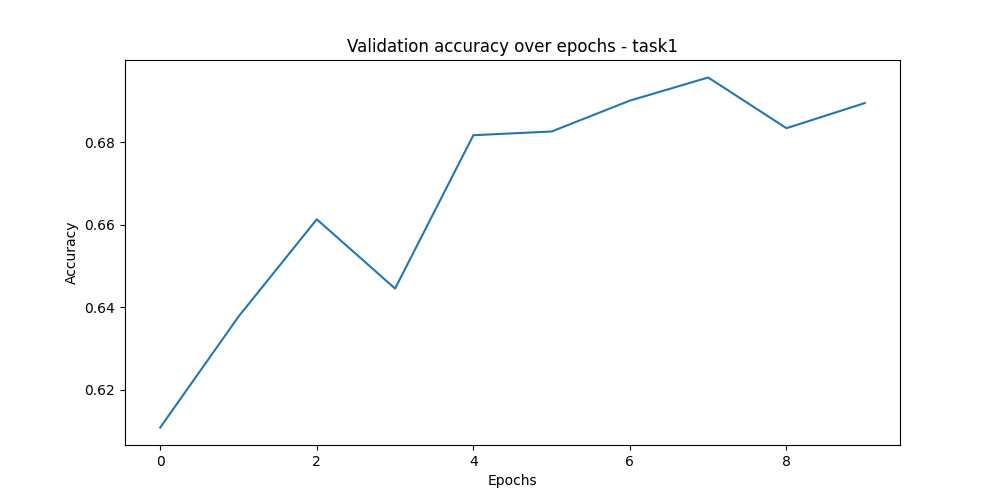
\includegraphics[width=0.8\textwidth]{accuracy_task1_num_filters_16.png}
  \caption{Accuracy over epochs for 16 filters}
\end{figure}

\begin{figure}[H]
  \centering
  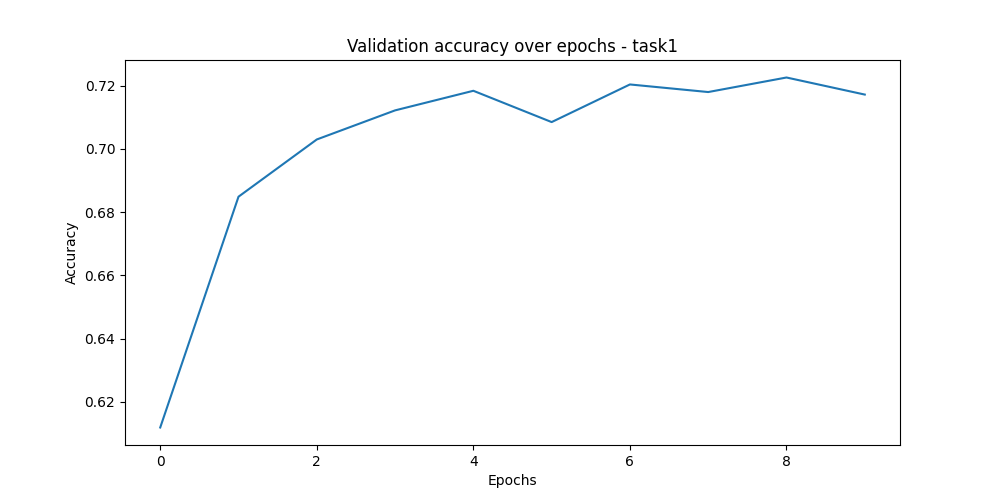
\includegraphics[width=0.8\textwidth]{accuracy_task1_num_filters_32.png}
  \caption{Accuracy over epochs for 32 filters}
\end{figure}

The model with 32 filters performed better than the model with 16 filters. It ended with an accuracy of 0.72 vs 0.69.

\section{Task 2}

The following are plots of accuracy over epochs for kernel sizes of 3 and 5 respectively.

\begin{figure}[H]
  \centering
  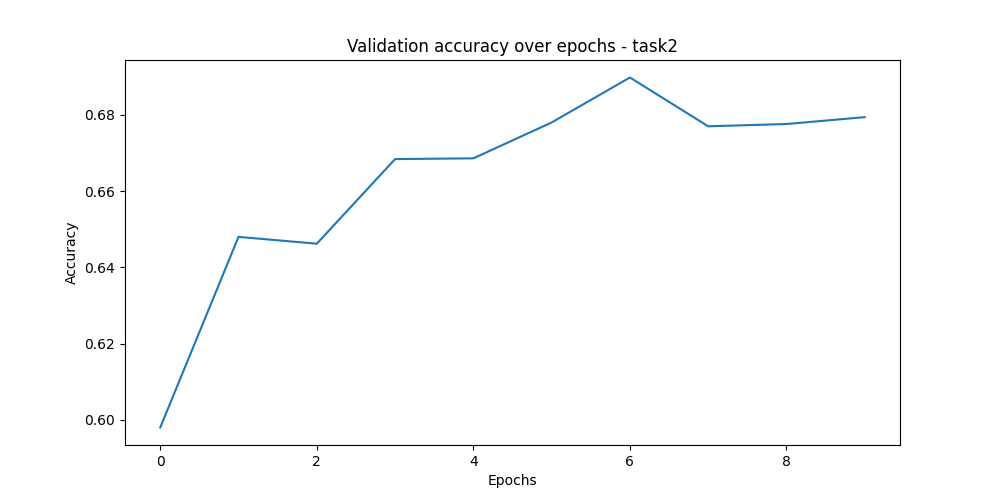
\includegraphics[width=0.8\textwidth]{accuracy_task2_kernel_size_3.png}
  \caption{Accuracy over epochs for kernel size 3}
\end{figure}

\begin{figure}[H]
  \centering
  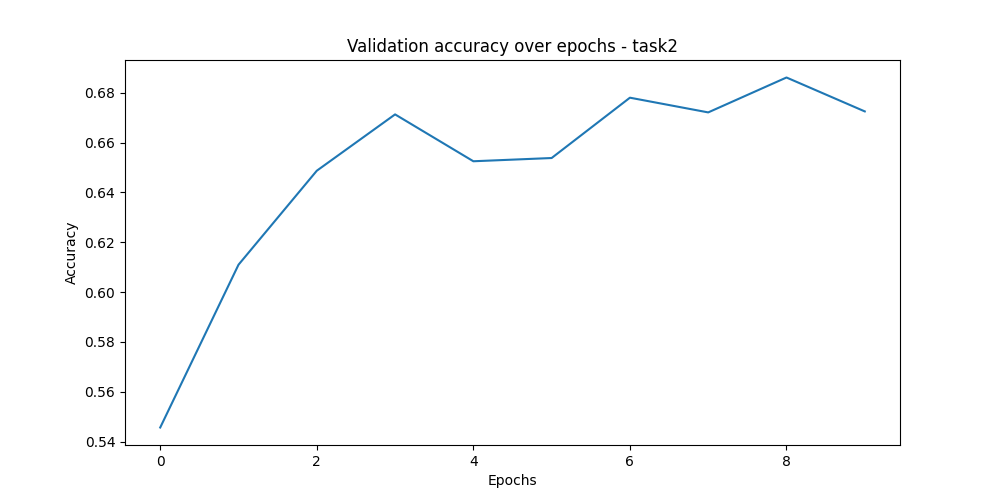
\includegraphics[width=0.8\textwidth]{accuracy_task2_kernel_size_5.png}
  \caption{Accuracy over epochs for kernel size 5}
\end{figure}

The models performed very similarly, with the model with kernel size 3 ending with an accuracy of 0.68 and the model with kernel size 5 ending with an accuracy of 0.67.

\newpage

\section{Task 3}

The following are plots of accuracy over epochs for padding and no padding respectively.

\begin{figure}[H]
  \centering
  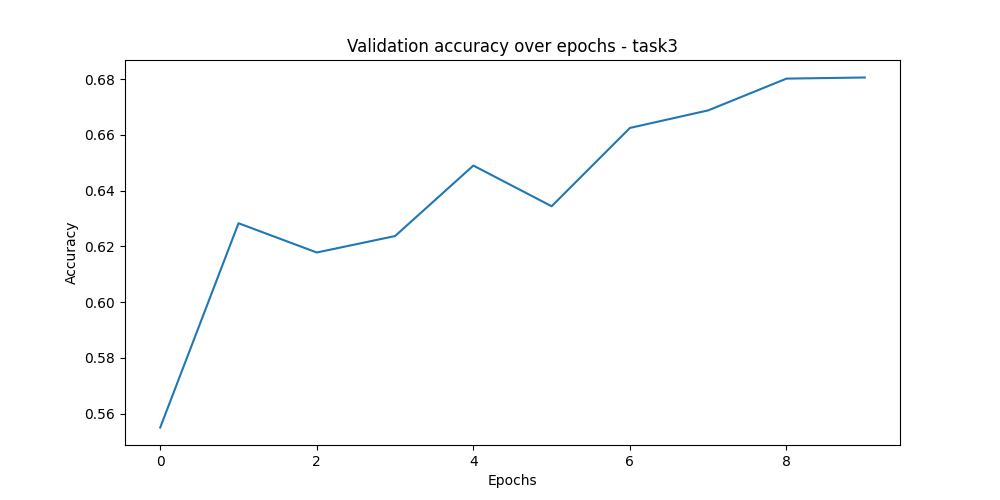
\includegraphics[width=0.8\textwidth]{accuracy_task3_padding_0.png}
  \caption{Accuracy over epochs for no padding}
\end{figure}

\begin{figure}[H]
  \centering
  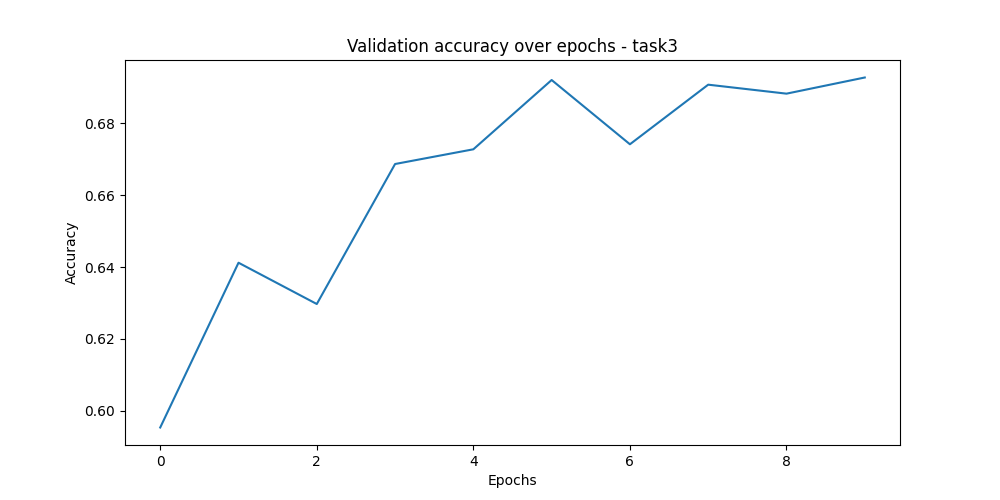
\includegraphics[width=0.8\textwidth]{accuracy_task3_padding_1.png}
  \caption{Accuracy over epochs for padding}
\end{figure}

Once again, the models performed very similarly, with the model with no padding ending with an accuracy of 0.68 and the model with padding ending with an accuracy of 0.69.

\newpage

\section{Task 4}

The following is a plot of accuracy over epochs for the best model.
The settings used were 32 filters, kernel size 3, and padding.

\begin{figure}[H]
  \centering
  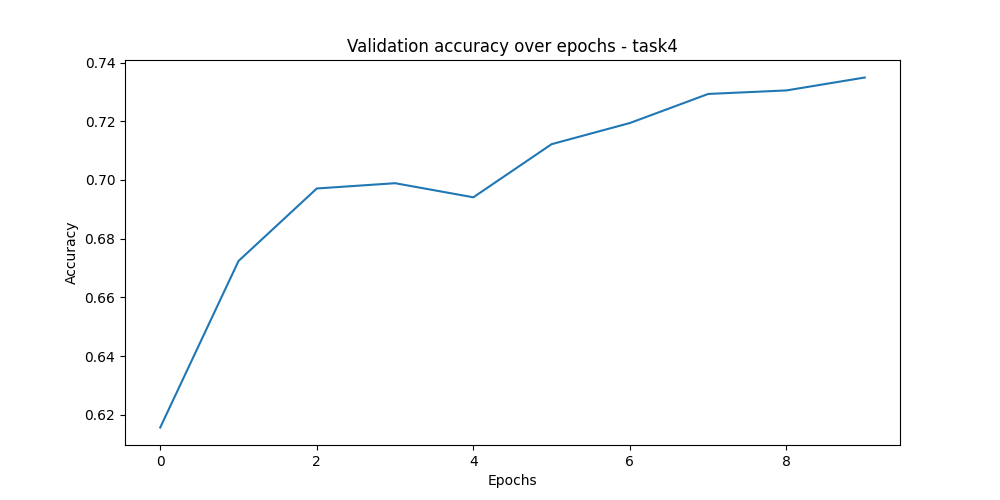
\includegraphics[width=0.8\textwidth]{accuracy_task4_num_filters_32_kernel_size_3_padding_1_dropout_rate_0.3.png}
  \caption{Accuracy over epochs for the best model}
\end{figure}

The accuracy of the best model was 0.74, which is the highest accuracy of all the models so far.

\end{document}